%\documentclass[10pt,reqno]{amsart}
\documentclass{article}
\usepackage[centertags]{amsmath}
\usepackage{amsfonts}
\usepackage{amssymb}
\usepackage{amsthm}
\usepackage{newlfont}
\usepackage{amscd}
\usepackage[all,cmtip]{xy}
\usepackage[pagebackref=false,colorlinks]{hyperref}
\usepackage{mathrsfs}
\usepackage{fancyhdr}
\hypersetup{pdffitwindow=true,linkcolor=blue,citecolor=blue,urlcolor=cyan}
% \usepackage{kotex}

\addtolength{\textwidth}{3cm}
\addtolength{\textheight}{3cm}
\addtolength{\hoffset}{-1.5cm}
\addtolength{\voffset}{-1.5cm}


% THEOREM Environments---------------------------------------------------

% MATH -------------------------------------------------------------------
\theoremstyle{remark}
\newtheorem{thm}{Theorem}
\newtheorem{cor}[thm]{Corollary}
\newtheorem{lem}[thm]{Lemma}
\newtheorem{prop}[thm]{Proposition}


\pagestyle{plain}
\usepackage{graphicx}
\graphicspath{ {./images/} }
\usepackage{wrapfig}
\usepackage{lipsum}


\title{A ``Good" Code for Free}
\author{Scott Stetson}
\date{October 15$^\text{th}$ 2022}

\begin{document}
	\maketitle
	One of the main problems in Coding Theory is to find the largest code with length $n$ and minimum Hamming distance $d$.  A code consists of codewords, strings or vectors, of a fixed length $n$ and the Hamming distance between two codewords is the number of coordinates in which they differ.  For example the Hamming distance between codewords $0011$ and $1001$ is two since only their first and third entries differ.  A code is said to have a minimum Hamming distance of $d$ if given any two codewords in the code, their Hamming distance is at least $d$.  An $(n,M,d)$ code is a code with $M$ codewords, each of length $n$, and with minimum Hamming distance $d$.
	Now that we have our notations we can represent the problem mathematically.  For $n$ and $d$ fixed, what is the largest value of $M$, i.e., how large can you make the code?  Let $A_2(n,d)$ be this maximum for binary codes.
	
	By a brute force search one can show that $A_2(9,6)=4$ and one such code is given below
	\begin{align*}
		c_1 & =100010110 \;\;\;\;\;\; c_3=101001001 \nonumber \\
		c_2 & =010100101 \;\;\;\;\;\; c_4=011111010
	\end{align*}
	However as $n$ and $d$ increase, the brute force method becomes computationally infeasible and clever methods are needed.  There are certain values for which $A_2(n,d)$ is known, see the following table and Brouwer's Table \cite{Brouwer} for more values.
	
	\begin{center}
		{\renewcommand{\arraystretch}{1.15}
		\begin{tabular}{|c|c|c|c|c|}
			\hline
			$n$ & $d=4$ & $d=6$ & $d=8$ & $d=10$ \\
			\hline
			$6$ & $4$ & $2$ & $1$ & $1$ \\
			\hline
			$7$ & $8$ & $2$ & $1$ & $1$ \\
			\hline
			$8$ & $16$ & $2$ & $2$ & $1$ \\
			\hline
			$9$ & $20$ & $4$ & $2$ & $1$ \\
			\hline
			$10$ & $40$ & $6$ & $2$ & $2$ \\
			\hline
			$11$ & $72$ & $12$ & $2$ & $2$ \\
			\hline
			$12$ & $144$ & $24$ & $4$ & $2$ \\
			\hline
			$13$ & $256$ & $32$ & $4$ & $2$ \\
			\hline
			$14$ & $512$ & $64$ & $8$ & $2$ \\
			\hline
			$15$ & $1024$ & $128$ & $16$ & $4$ \\
			\hline
			$16$ & $2048$ & $256$ & $32$ & $4$ \\
			\hline
			$17$ & $2816-3276$ & $258-340$ & $36$ & $6$ \\
			\hline
			$18$ & $5632-6552$ & $512-673$ & $64$ & $10$ \\
			\hline
		\end{tabular}
	}
	\end{center}
	The function $A_2$ satisfies the identity that $A_2(n-1,2e-1)=A_2(n,2e)$ which is why only even distances are listed in the columns above.  The entries where two numbers are listed represent the upper and lower bounds for the value of $A_2(n,d)$.  Take for example $A_2(17,6)$ whose entry is $258-340$
	\begin{equation*}
		\Rightarrow 258\leq A_2(17,6)\leq 340
	\end{equation*}
	and this value of $A_2$ is the reason why I am writing this paper.  The lower bound was improved to 258 in 2018 by Moshe Milshtein \cite{Milshtein} who found a (16,258,5) code.  One way to show a greater lower bound is to explicitly give a code that achieves it, and recall that $A_2(17,6)=A_2(16,5)$.  Now what was the bound before 258?  It was 256 and it had been  since 1967 when Nordstrom and Robinson \cite{NS} constructed their (15,256,5) optimal code.  So it took 51 years to improve the lower bound of $A_2(16,5)$ which shows that in general this problem is very hard.  Also note that even though $A_2(15,5)\neq A_2(16,5)$ it is true that $A_2(15,5)\leq A_2(16,5)$ since one can take the Nordstrom Robinson code and add a zero to the end of each codeword thereby increasing the length while keeping the same Hamming distance between all codewords.  It turns out that there is a very simple way to find a (16,256,5) code, but first let's look further into the Nordstrom Robinson code to see their construction.
	
	In \cite{NS} each codeword has 15 bits labeled $X_0X_1X_2X_3X_4X_5X_6X_7Y_0Y_1Y_2Y_3Y_4Y_5Y_6$ where the $X$'s are the information bits, which run through all $2^8=256$ possibilities, and the $Y$'s are the redundant bits.  $Y_0$ is defined as
	\begin{align}
		Y_0=X_7\oplus X_6\oplus X_0\oplus X_1\oplus X_3 & \oplus (X_0\oplus X_4)(X_1\oplus X_2\oplus X_3\oplus X_5) \nonumber \\
		& \oplus(X_1\oplus X_2)(X_3\oplus X_5)
	\end{align}
	where $\oplus$ denotes modulo 2 addition, i.e., the remainder after dividing by 2
	\begin{align*}
		0\oplus0 & =0 \\
		0\oplus1 & =1 \\
		1\oplus0 & =1 \\
		1\oplus1 & =0.
	\end{align*}
	Quoting \cite{NS}, the remaining $Y$'s are found by cyclically shifting $X_0$ through $X_6$; i.e., for $Y_j$ substitute $X_{i+j(\text{mod }7)}$ for $X_i$ in (1) where $i=0,1,\dots,6$ for each $i,j=0,1,\dots,6$.
	
	The construction of this code is not simple by any means and I'm guessing that it took Nordstrom and Robinson a while to come up with these formulas.  Now we get to the interesting, but mostly hilarious part, at least to me.  Back to $(16,M,5)$ codes, as I mentioned before one can use the Nordstrom Robinson code to construct a $(16,256,5)$ code, but you can also find one in the following way:
	\begin{enumerate}
		\item For the numbers 0 to 256 write them in their binary form and pad them with zeros on the left until the result is a codeword of length 16.  This is just generating all $2^{16}=65,536$ possible codewords.
		\item Start off with $C=\{\textbf{0}\}$, the all zero codeword.  Sequentially look at the next codeword, $c_i$, add it to the code if the Hamming distance between $c_i$ and $c_j$ is greater than or equal to 5 for all $c_j\in C$.
	\end{enumerate}

	\noindent Let's run through a couple of steps to see how this works.  Starting off we have
	\begin{equation*}
		C=\{0000000000000000\}.
	\end{equation*}
	The next codeword is $0000000000000001$ which has a Hamming distance of only 1 from the all zero codeword so we do not add it to our code.  Remember that we are constructing a $(16,256,5)$ code, so any and all codewords in our code must have a Hamming distance of at least 5.  Next we turn to $0000000000000010$ which is just two in binary padded with zeros on the left.  Again the Hamming distance between this codeword and the one with all zeros is only 1 so we do not add it to our code $C$.  In fact in order for us to add a codeword to our code it must have at least 5 ones.  The first time this happens is for the number 31 since $1+2+2^2+2^3+2^4=31$ so we have
	\begin{equation*}
		C=\{0000000000000000,0000000000011111\}.
	\end{equation*}
	Continuing the next codeword is $0000000000100000$ but this codeword does not have 5 ones so we do not add it to our code.  Eventually we arrive at $0000000000101111$, the binary representation of 47, which has 5 ones, but the Hamming distance between $0000000000101111$ and $0000000000011111$ is only 2 so we do not add this to our code.  $C$ stays at size 2 until we arrive at 227, then we have
	\begin{equation*}
		C=\{0000000000000000,0000000000011111,0000000011100011\}.
	\end{equation*}
	Of course this method ends after checking all $2^{16}$ possibilities and we are left with a $(16,256,5)$ code.  The explanation above may seem long, but I am trying to be very clear for those who have never seen this before.  Turning now to mathematical notation we see it's power in the following Mathematica program which is one way to generate this code $C$.
	\begin{center}
		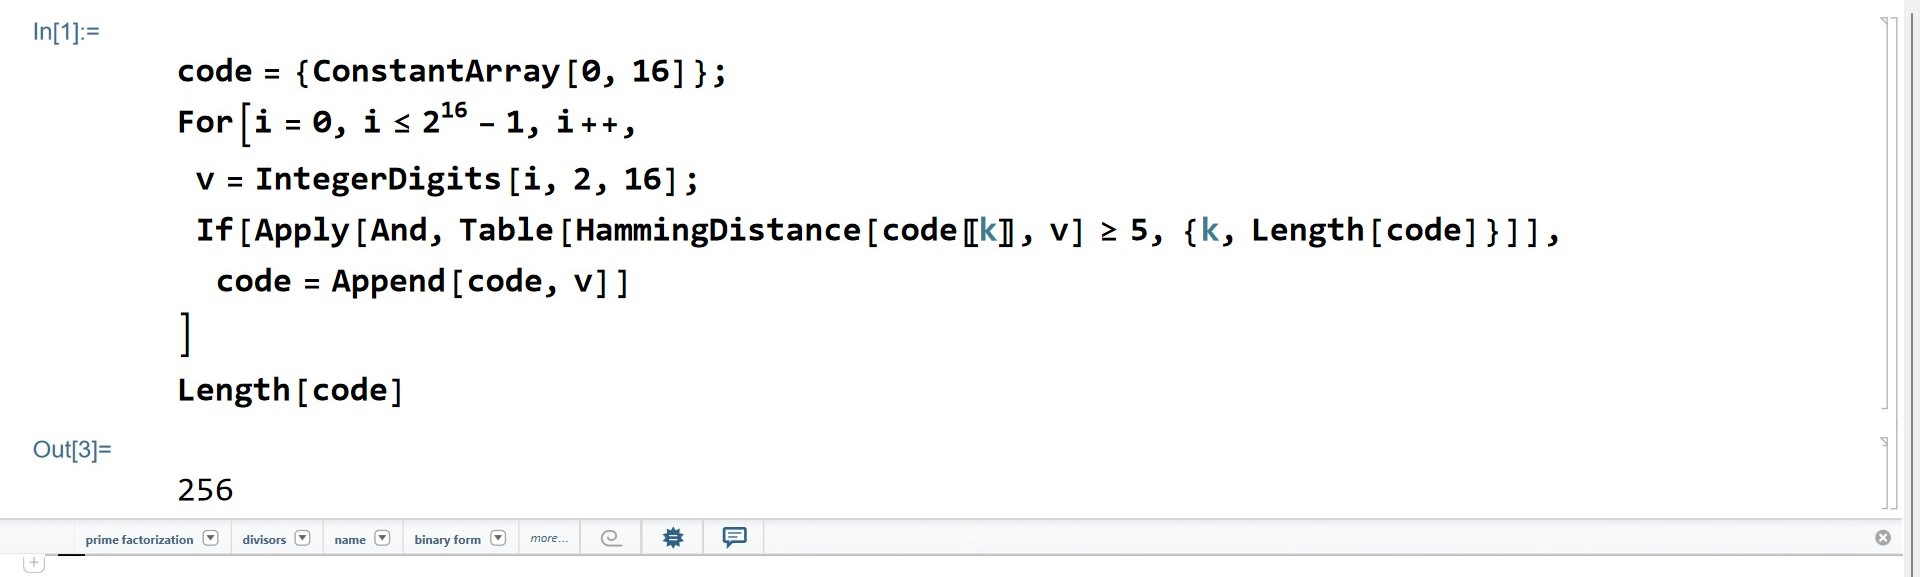
\includegraphics[width=15cm]{sequential code}
	\end{center}
	Notice that only the definition of an $(n,M,d)$ code is used in this program! I find it hilarious that everything just lined up and we get this ``good" code for free which was not surpassed for 51 years.  I use quotes around the word good because no one knows what the actual value of $A_2(16,5)$ is.  If $A_2(16,5)$ is actually 258 then it is a good code because 256 is close to 258.  But if $A_2(16,5)$ is closer to 300, then this code was good for a certain time.  The future will tell.
	
	One last thing before we conclude.  Looking at Brouwer's Table \cite{Brouwer} again we see that
	\begin{equation*}
		512\leq A_2(17,5)=A_2(18,6)\leq 673.
	\end{equation*}
	If we perform this sequential searching on codewords of length 17 we see that the code produced achieves this lower bound.
	\begin{center}
		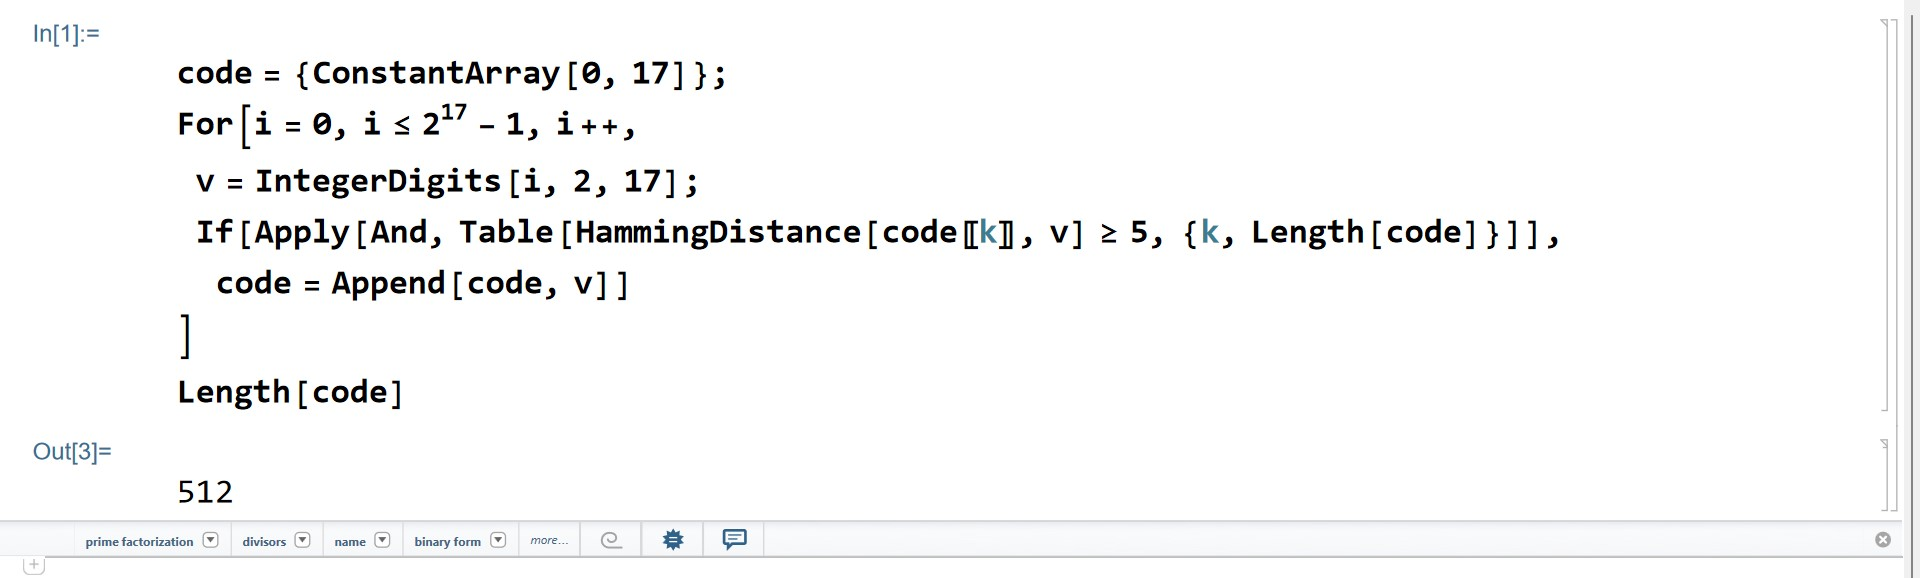
\includegraphics[width=15cm]{sequential code 512}
	\end{center}
	With all the algorithms out there, no one has been able to come up with a better $(17,M,5)$ code than the one given by sequentially running through all codewords and just checking the Hamming distance.
	\begin{thebibliography}{9}
		\bibitem{Brouwer}
		Brouwer's Table  \href{https://www.win.tue.nl/~aeb/codes/binary-1.html}{https://www.win.tue.nl/$\sim$aeb/codes/binary-1.html}
		
		\bibitem{Milshtein}
		Milshtein, M. A new two-error-correcting binary code of length 16. Cryptogr. Commun. 12, 71–75 (2020). \href{https://doi.org/10.1007/s12095-019-00365-7}{https://doi.org/10.1007/s12095-019-00365-7}
		
		\bibitem{NS}
		 A. W. Nordstrom and J. P. Robinson, \textit{An optimum nonlinear code}, Inform. Control,
		11 (1967), 613–61
	\end{thebibliography}
	
	
	
\end{document}